\section{Optimizacijska nivelacija uzdužnog profila ceste primjenom linearnog programiranja}

\subsection{Kontinuirana varijacijska formulacija problema}

U građevinarstvu i prometnom inženjerstvu projektiranje uzdužnog profila prometnice predstavlja temeljni optimizacijski zadatak. Cilj je odrediti visinsku trasu ceste $y(x)$ koja minimizira ukupne zemljane radove (volumen iskopa i nasipa), uz istovremeno zadovoljavanje prometno-tehničkih standarda: maksimalnog uzdužnog nagiba i maksimalne zakrivljenosti trase (udobnost vožnje i ograničenje vertikalnih akceleracija)~\cite{jokic2024predavanja}.

Neka je $L$ horizontalna duljina dionice ceste ($x \in [0, L]$), a $h(x)$ poznata prirodna visina terena. Uz pretpostavku jedinične širine poprečnog presjeka ceste ($w = 1\text{ m}$), ukupni volumen zemljanih radova $[\text{m}^3]$ izravno odgovara površini uzdužnog presjeka $[\text{m}^2]$ između nivelete ceste $y(x)$ i prirodnog terena $h(x)$. Problem se kontinuirano formulira kao varijacijski optimizacijski problem:
\begin{equation}
\min_{y(x)} \quad J[y] = \int_0^L |y(x) - h(x)| \, dx
\label{eq:road_continuous}
\end{equation}
uz ograničenja:
\begin{align}
|y'(x)| &\leq b_1, \quad \forall x \in [0, L], \label{eq:road_slope_cont} \\
|y''(x)| &\leq b_2, \quad \forall x \in [0, L], \label{eq:road_curv_cont} \\
y(0) &= a, \quad y(L) = b. \label{eq:road_bc_cont}
\end{align}

Zadani parametri modela su:
\begin{equation}
L = 10 \text{ m}, \quad h(x) = 0.0053 x^4 - 0.095 x^3 + 0.48 x^2 - 0.3 x + 1,
\end{equation}
\begin{equation}
a = h(0) = 1 \text{ m}, \quad b = h(L) = 4 \text{ m}.
\end{equation}
Razmatraju se dva skupa parametara:
\begin{itemize}
    \item \textbf{Slučaj A}: $b_1 = 0.5$ (maksimalni nagib $[\text{m/m}]$), $b_2 = 0.5 \text{ m}^{-1}$ (maksimalna zakrivljenost).
    \item \textbf{Slučaj B}: $b_1 = 0.5$ (maksimalni nagib $[\text{m/m}]$), $b_2 = 0.2 \text{ m}^{-1}$ (stroži uvjet zakrivljenosti / udobnosti vožnje).
\end{itemize}

\subsection{Diskretizacija konačnim razlikama}

Područje $[0, L]$ diskretizira se s $N$ jednakih podintervala duljine $\Delta x = L/N$, čime se dobiva mreža od $N+1$ čvorova:
\begin{equation}
x_i = i \cdot \Delta x, \quad i = 0, 1, \dots, N, \quad \text{pri čemu je } x_0 = 0, \; x_N = L.
\end{equation}
Vektor visina terena u čvorovima označavamo s $h = [h_0, h_1, \dots, h_N]^T \in \mathbb{R}^{N+1}$, gdje je $h_i = h(x_i)$.

Vektor nepoznatih visina nivelete ceste u diskretnim čvorovima je $y = [y_0, y_1, \dots, y_N]^T \in \mathbb{R}^{N+1}$.

\subsubsection{Aproksimacija prve i druge derivacije}

Prema uputama zadatka, nagib ceste u čvorovima aproksimira se prvom unazadnom podijeljenom razlikom:
\begin{equation}
y'(x_i) \approx \nabla y_i = \frac{y_i - y_{i-1}}{\Delta x}, \quad i = 1, \dots, N.
\label{eq:diff_first}
\end{equation}
Brzina promjene nagiba (druga podijeljena razlika / aproksimacija vertikalne zakrivljenosti za male nagibe, $y''$) aproksimira se drugom podijeljenom razlikom:
\begin{equation}
y''(x_i) \approx \nabla^2 y_i = \frac{\nabla y_i - \nabla y_{i-1}}{\Delta x} = \frac{y_i - 2y_{i-1} + y_{i-2}}{\Delta x^2}, \quad i = 2, \dots, N.
\label{eq:diff_second}
\end{equation}

U matričnom zapisu diferencijalni operatori glase:
\begin{equation}
\nabla y = D_1 y \in \mathbb{R}^N, \quad \nabla^2 y = D_2 y \in \mathbb{R}^{N-1},
\end{equation}
gdje su matrice konačnih razlika $D_1 \in \mathbb{R}^{N \times (N+1)}$ i $D_2 \in \mathbb{R}^{(N-1) \times (N+1)}$ definirane kao:
\begin{equation}
D_1 = \frac{1}{\Delta x} \begin{bmatrix}
-1 & 1 & 0 & \dots & 0 & 0 \\
0 & -1 & 1 & \dots & 0 & 0 \\
\vdots & \vdots & \ddots & \ddots & \vdots & \vdots \\
0 & 0 & \dots & -1 & 1 & 0 \\
0 & 0 & \dots & 0 & -1 & 1
\end{bmatrix},
\end{equation}
\begin{equation}
D_2 = \frac{1}{\Delta x^2} \begin{bmatrix}
1 & -2 & 1 & 0 & \dots & 0 & 0 \\
0 & 1 & -2 & 1 & \dots & 0 & 0 \\
\vdots & \vdots & \ddots & \ddots & \ddots & \vdots & \vdots \\
0 & 0 & \dots & 1 & -2 & 1 & 0 \\
0 & 0 & \dots & 0 & 1 & -2 & 1
\end{bmatrix}.
\end{equation}

\subsection{Transformacija u standardni oblik linearnog programa (LP)}

Diskretizirani integralni kriterij glasi:
\begin{equation}
J_{\mathrm{disc}}[y] = \Delta x \sum_{i=0}^N |y_i - h_i|,
\label{eq:road_disc_obj}
\end{equation}
pri čemu $\Delta x$ predstavlja korak pravokutne numeričke integracije (Riemannova suma) površine uzdužnog presjeka.

Zbog prisutnosti nelinearnog operatora apsolutne vrijednosti ($|y_i - h_i|$), problem se prevodi u linearni program primjenom metode epigrafskih pomoćnih varijabli $z_i \geq |y_i - h_i|$~\cite{boyd2004convex,nocedal2006numerical}.

Za svaki čvor $i = 0, \dots, N$ nejednakost $z_i \geq |y_i - h_i|$ ekvivalentna je paru linearnih nejednakosti:
\begin{align}
y_i - z_i &\leq h_i, \label{eq:lp_slack1} \\
-y_i - z_i &\leq -h_i. \label{eq:lp_slack2}
\end{align}
Prošireni vektor optimizacijskih varijabli $\theta \in \mathbb{R}^{2N+2}$ definira se kao:
\begin{equation}
\theta = \begin{bmatrix} y \\ z \end{bmatrix} = \begin{bmatrix} y_0 & y_1 & \dots & y_N & z_0 & z_1 & \dots & z_N \end{bmatrix}^T.
\end{equation}

Funkcija cilja linearnog programa glasi:
\begin{equation}
\min_{\theta \in \mathbb{R}^{2N+2}} \quad f_{\mathrm{LP}}^T \theta = \Delta x \sum_{i=0}^N z_i = \begin{bmatrix} \mathbf{0}_{1 \times (N+1)} & \Delta x \cdot \mathbf{1}_{1 \times (N+1)} \end{bmatrix} \begin{bmatrix} y \\ z \end{bmatrix}.
\end{equation}

\subsubsection{Struktura matrice nejednakosti $A_{\mathrm{ineq}} \theta \leq b_{\mathrm{ineq}}$}

Sustav linearnih nejednakosti objedinjuje tri grupe fizikalnih ograničenja:
\begin{enumerate}
    \item \textbf{Epigrafska ograničenja apsolutnog odstupanja} ($2(N+1)$ nejednakosti):
    \begin{equation}
    \begin{bmatrix} I_{N+1} & -I_{N+1} \\ -I_{N+1} & -I_{N+1} \end{bmatrix} \begin{bmatrix} y \\ z \end{bmatrix} \leq \begin{bmatrix} h \\ -h \end{bmatrix}.
    \end{equation}
    \item \textbf{Ograničenja nagiba} ($2N$ nejednakosti):
    \begin{equation}
    \begin{bmatrix} D_1 & \mathbf{0}_{N \times (N+1)} \\ -D_1 & \mathbf{0}_{N \times (N+1)} \end{bmatrix} \begin{bmatrix} y \\ z \end{bmatrix} \leq \begin{bmatrix} b_1 \mathbf{1}_N \\ b_1 \mathbf{1}_N \end{bmatrix}.
    \end{equation}
    \item \textbf{Ograničenja zakrivljenosti} ($2(N-1)$ nejednakosti):
    \begin{equation}
    \begin{bmatrix} D_2 & \mathbf{0}_{(N-1) \times (N+1)} \\ -D_2 & \mathbf{0}_{(N-1) \times (N+1)} \end{bmatrix} \begin{bmatrix} y \\ z \end{bmatrix} \leq \begin{bmatrix} b_2 \mathbf{1}_{N-1} \\ b_2 \mathbf{1}_{N-1} \end{bmatrix}.
    \end{equation}
\end{enumerate}
Ukupan broj linearnih nejednakosti u matrici $A_{\mathrm{ineq}}$ iznosi:
\begin{equation}
N_{\mathrm{ineq}} = 2(N+1) + 2N + 2(N-1) = 6N.
\end{equation}

\subsubsection{Struktura matričnih jednakosti $A_{\mathrm{eq}} \theta = b_{\mathrm{eq}}$}

Rubni uvjeti u točkama $x=0$ i $x=L$ zapisuju se kao sustav od 2 linearne jednakosti:
\begin{equation}
\begin{bmatrix}
1 & 0 & \dots & 0 & \mathbf{0}_{1 \times (N+1)} \\
0 & \dots & 0 & 1 & \mathbf{0}_{1 \times (N+1)}
\end{bmatrix} \begin{bmatrix} y \\ z \end{bmatrix} = \begin{bmatrix} 1 \\ 4 \end{bmatrix}.
\end{equation}
Donja granica za varijable je $z_i \geq 0$, dok su varijable $y_i$ slobodne ($-\infty < y_i < \infty$).

\subsection{Numerički rezultati za četiri ispitna slučaja}

Problem je riješen primjenom optimizacijskog algoritma dualnog simpleksa (\texttt{linprog} s opcijom \texttt{dual-simplex} i \texttt{highs}) za četiri zahtijevana scenarija:
\begin{enumerate}
    \item \textbf{Slučaj A, $N=20$}: $b_1 = 0.5$, $b_2 = 0.5 \text{ m}^{-1}$, $\Delta x = 0.5 \text{ m}$ ($42$ varijable, $120$ nejednakosti).
    \item \textbf{Slučaj A, $N=100$}: $b_1 = 0.5$, $b_2 = 0.5 \text{ m}^{-1}$, $\Delta x = 0.1 \text{ m}$ ($202$ varijable, $600$ nejednakosti).
    \item \textbf{Slučaj B, $N=20$}: $b_1 = 0.5$, $b_2 = 0.2 \text{ m}^{-1}$, $\Delta x = 0.5 \text{ m}$ ($42$ varijable, $120$ nejednakosti).
    \item \textbf{Slučaj B, $N=100$}: $b_1 = 0.5$, $b_2 = 0.2 \text{ m}^{-1}$, $\Delta x = 0.1 \text{ m}$ ($202$ varijable, $600$ nejednakosti).
\end{enumerate}

Sintetički prikaz optimalnih rezultata dan je u tablici~\ref{tab:road_results}.

\begin{table}[H]
\centering
\caption{Numerički rezultati optimalne nivelacije ceste za Slučaje A i B.}
\label{tab:road_results}
\begin{tabular}{lcccccc}
\toprule
\textbf{Slučaj} & $N$ & $\Delta x$ [m] & \textbf{Ukupni trošak $J^*$ [$\text{m}^2$]} & \textbf{Iskop [$\text{m}^2$]} & \textbf{Nasip [$\text{m}^2$]} & $\max |y''|$ [$\text{m}^{-1}$] \\
\midrule
A & 20 & 0.5 & 1.916180 & 0.0877 & 1.8285 & 0.5000 \\
A & 100 & 0.1 & 1.965940 & 0.1287 & 1.8372 & 0.5000 \\
B & 20 & 0.5 & 2.453727 & 0.3026 & 2.1511 & 0.2000 \\
B & 100 & 0.1 & 2.506047 & 0.2645 & 2.2416 & 0.2000 \\
\bottomrule
\end{tabular}
\end{table}

\begin{figure}[H]
    \centering
    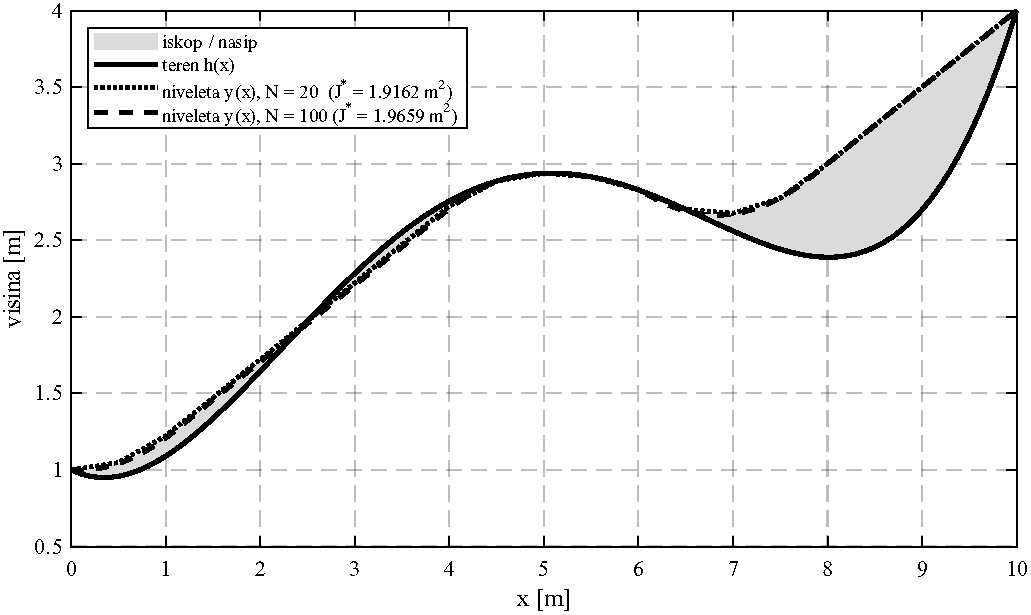
\includegraphics[width=0.88\textwidth]{figures/fig3_1_road_case_A.pdf}
    \caption{Optimalni uzdužni profil ceste $y(x)$ za Slučaj A ($b_1 = 0.5, b_2 = 0.5$) s označenim zonama iskopa i nasipa.}
    \label{fig:road_case_a}
\end{figure}

\begin{figure}[H]
    \centering
    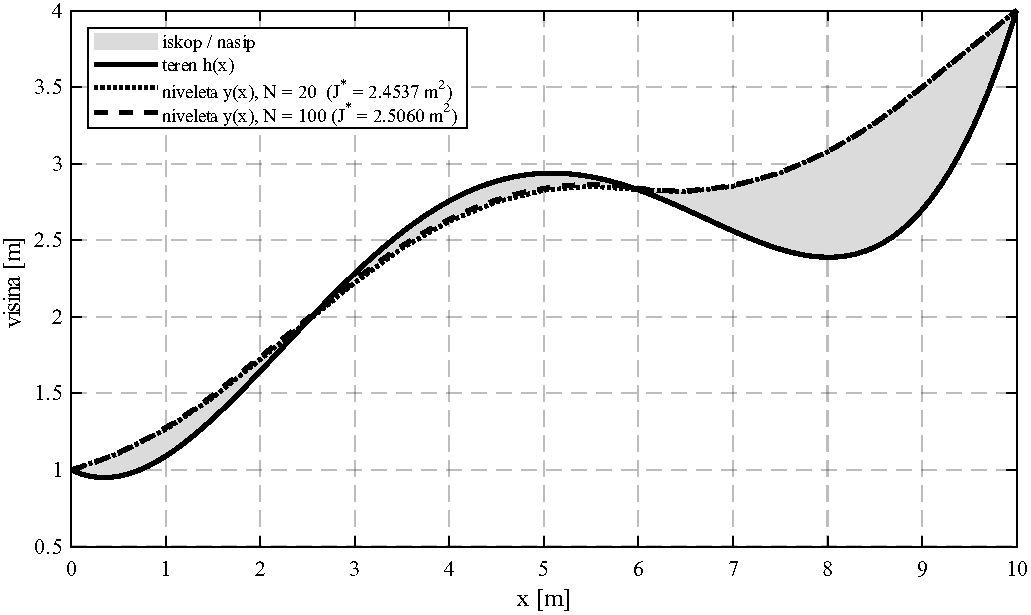
\includegraphics[width=0.88\textwidth]{figures/fig3_2_road_case_B.pdf}
    \caption{Optimalni uzdužni profil ceste $y(x)$ za Slučaj B ($b_1 = 0.5, b_2 = 0.2$) uz strože ograničenje zakrivljenosti.}
    \label{fig:road_case_b}
\end{figure}

\subsection{Analiza utjecaja gustoće diskretizacije i parametara ograničenja}

Usporedba grafova na slikama~\ref{fig:road_case_a} i~\ref{fig:road_case_b} te provjere derivacija na slikama~\ref{fig:road_slope} i~\ref{fig:road_curv} pokazuju sljedeće zakonitosti:

\begin{enumerate}
    \item \textbf{Utjecaj gustoće diskretizacije ($N = 20$ vs $N = 100$)}:
    Povećanjem broja diskretizacijskih točaka s $N=20$ na $N=100$, diskretni integral $J_{\mathrm{disc}}$ asimptotski konvergira prema kontinuiranom integralu $\int_0^L |y(x)-h(x)|dx$. Za Slučaj A vrijednost raste s $1.9162$ na $1.9659 \text{ m}^2$ ($+2.59\%$), dok za Slučaj B raste s $2.4537$ na $2.5060 \text{ m}^2$ ($+2.13\%$). Fina mreža omogućuje vjernije praćenje promjena profila bez numeričkog izglađivanja.
    
    \item \textbf{Utjecaj ograničenja zakrivljenosti ($b_2 = 0.5$ vs $b_2 = 0.2$)}:
    Smanjenje dozvoljene zakrivljenosti s $b_2 = 0.5 \text{ m}^{-1}$ (Slučaj A) na $b_2 = 0.2 \text{ m}^{-1}$ (Slučaj B) zahtijeva znatno glađu trasu ceste. Posljedično, niveleta ne može pratiti prirodne pregibe terena, što povećava ukupni volumen zemljanih radova s $1.9659 \text{ m}^2$ na $2.5060 \text{ m}^2$ ($+27.47\%$).
\end{enumerate}

\begin{figure}[H]
    \centering
    \includegraphics[width=0.85\textwidth]{figures/fig3_3_road_slope_profile.pdf}
    \caption{Provjera ograničenja prvog reda: profil nagiba ceste $y'(x)$ duž trase za Slučaje A i B.}
    \label{fig:road_slope}
\end{figure}

\begin{figure}[H]
    \centering
    \includegraphics[width=0.85\textwidth]{figures/fig3_4_road_curvature_profile.pdf}
    \caption{Provjera ograničenja drugog reda: profil zakrivljenosti $y''(x)$ i zasićenje na granicama $\pm b_2$.}
    \label{fig:road_curv}
\end{figure}

Na slici~\ref{fig:road_curv}, numerička aproksimacija druge derivacije $y''(x)$ u Slučaju B doseže točno ekstremne vrijednosti $\pm 0.2 \text{ m}^{-1}$, potvrđujući da su ograničenja drugog reda aktivna duž značajnih segmenata trase.
